\newpage
\section{Exercises}

\subsection{Partie 1}

Voici un ensemble d'exercices utilisants les principes de base du C\#.
Il ne sont \textbf{pas} triés par ordre de difficulté. Si vous êtes bloqués, demandez de
l'aide aux assistants.

\subsubsection{Fibonacci}

Le but de ce premier exercice est d'implémenter la suite de Fibonacci en C\#.
Pour rappel, la suite de Fibonacci est définie comme suit:

$$
\mathcal{F}_0 = 0\\
$$
$$
\mathcal{F}_1 = 1\\
$$
$$
\mathcal{F}_{n+2} = \mathcal{F}_{n} + \mathcal{F}_{n + 1}
$$

\begin{code}
private static long Fibo(long n)
{
	// TODO
    return 0;
}
\end{code}

\subsubsection{Factorielle}

Pour cet exercice, vous devez implémenter la fonction factorielle.

Pour rappel, factorielle est décrite comme suit:

$$
\mathcal{T}(0) = 1
$$
$$
\mathcal{T}(n) = n \times \mathcal{T}(n - 1)
$$

\begin{code}
private static long Fact(long n)
{
	// TODO
    return 0;
}
\end{code}

\subsubsection{Swapons}

Pour cet exercice, vous allez devoir utiliser les références.
Le but est d'échanger les valeurs de \(x\) et de \(y\).

\begin{code}
private static void Swap(ref int x, ref int y)
{
	// TODO
}
\end{code}

\subsubsection{MinTab}

Nous allons utiliser les tableaux. Votre but est de trouver la plus petite valeur
dans un tableau de \textbf{long}.

\begin{code}
private static long MinTab(long[] tab)
{
	// TODO
    return 0;
}
\end{code}

\subsubsection{Sum}

Il est possible en C\# de déclarer des matrices. 
Par exemple, pour déclarer la matrice identité de taille 3:

\begin{code}
int[,] identity3 = new int[,]
{
    {1, 0, 0},
    {0, 1, 0},
    {0, 0, 1}
};
\end{code}

Pour cet exercice, vous devez calculer la somme de deux matrices de même dimension.

Rappel:

$$
\mathcal{A} + \mathcal{B} = \begin{pmatrix}
   a_{11} & a_{12}  & \dots & a_{1n}\\
   a_{21} & a_{22}  & \dots & a_{2n}\\
   \vdots & \vdots & \ddots & \vdots \\
   a_{m1} & a_{m2} & \dots &  a_{mn}
 \end{pmatrix} + \begin{pmatrix}
   b_{11} & b_{12}  & \dots & b_{1n}\\
   b_{21} & b_{22}  & \dots & b_{2n}\\
   \vdots & \vdots & \ddots & \vdots \\
   b_{m1} & b_{m2} & \dots &  b_{mn}
 \end{pmatrix} = \begin{pmatrix}
   a_{11} + b_{11} & a_{12} + b_{12}  & \dots & a_{1n} + b_{1n}\\
   a_{21} + b_{21} & a_{22} + b_{22}  & \dots & a_{2n} + b_{2n}\\
   \vdots & \vdots & \ddots & \vdots \\
   a_{m1} + b_{m1} & a_{m2} + b_{m2} & \dots &  a_{mn} + b_{mn}
 \end{pmatrix}
$$

\begin{code}
private static long[,] Sum(long[,] mat1, long[,] mat2)
{
	long[,] matRes;
	// TODO
    return matRes;
}
\end{code}

\subsubsection{Parité}

Pour cet exercice, nous allons utiliser les \textbf{listes}. Vous devez vérifier qu'une liste donnée respecte la parité ou non.

On dit qu'une liste respecte la parité si elle est composée d'une alternance d'entiers pairs et impairs en commençant par un entier pair.

Par exemple:

\begin{code}
[4, 5, 8, -3, 2, 5] // Est une liste qui respecte la parité.
[4, 5, 8, -3, 1, 5] // N'est pas une liste qui respecte la parité.
[5, 8, -3, 2, 5, 4] // N'est pas une liste qui respecte la parité.
\end{code}

Voici le prototype de la fonction:
\begin{code}
private static bool Parite(List<int> list)
{
	// TODO
    return true;
}
\end{code}

\subsubsection{Bits Counter}

Vous devez compter le nombre de bits mis à \(1\) dans un nombre donné.

\textbf{Conseil}: Utilisez les opérateurs bitwise.

\begin{code}
private static uint NbBitsSet(long number)
{
	// TODO
    return 0;
}
\end{code}

\newpage
\subsection{Partie 2}

Les choses sérieuses vont commencer ! Vous allez devoir créer vos premières classes et objets.

Le but de cet exercice est d'implémenter 3 classes:
\begin{itemize}
\item Student 
\item ACDC 
\item Sup \\
\end{itemize}

Une fois que cela est fait, nous allons pouvoir faire combattre nos étudiants les uns
contre les autres.

\subsubsection{Student Constructor}

Vous l'avez compris vous allez implémenter votre premier constructeur. 
Mais avant cela, il faut définir les attributs de la classe.

Voici la liste des attributs et leur type:

\begin{itemize}
\item name : string
\item life : int
\item damage : int
\item is\_magician : bool
\item physical\_armor : int
\item magical\_armor : int\\
\end{itemize}

Vous pouvez mettre la protection des attributs à \textbf{public} pour le moment.

\begin{code}
class Student
{
	// Attributs (A vous de compléter)
    public string name_;
    // ...
    
    // Constructeur (A vous de compléter)
    public Student(string name, /* ... */)
    {
    	name_ = name;
        // ...
    }
}
\end{code}

\subsubsection{Take damage}

Maintenant que nos étudiants ont des attributs et peuvent être instanciés (construits), vous allez implémenter une méthode. 

La méthode \textbf{\texttt{TakeDamage}} va appliquer des dégâts (magiques ou physiques) à notre étudiant.

Voici la formule à appliquer:

$$
life = life - (damage - armor)
$$

Il faut compléter et modifier la formule de manière à respecter les points suivant:

\begin{itemize}
\item Armor dépend du type de dégât.
\item L'étudiant ne peut pas gagner de la vie.
\item L'étudiant ne peut pas avoir une vie négatif.
\end{itemize}


\begin{code}
public void TakeDamage(int damage, bool isMagical)
{	
	// TODO
}
\end{code}

\newpage
\subsection{Bonus}

\subsubsection{Print Int Array}

Le but de cet exercice est d'afficher dans la console l'intégralité d'un tableau d'entier.

Exemple :

\begin{code}
[0, 34, 5, 55, 666, 33, 23, 2] // Voici l'affichage attendu.
[7, 54, 55, 58, 996, 562, 0] // Voici un autre exemple.
\end{code}

Voici le prototype de la fonction:
\begin{code}
 static void print_array(int[] array)
{
	// TODO
}
\end{code}

Cet exercice va vous permettre de vérifier le tableau trié par l'algorithme qui suit.

\subsubsection{Insertion Sort}

Le but de cet exercice est d'implémenter un algorithme de tri par insertion.

\texttt{Insertion sort} est très simple : 

\begin{code}
Insertion Sort(int[] tab)
	Pour i allant de 0 à (taille du tableau - 1)
		min = tab[i]
        min_pos = i
        Pour j allant de (i + 1) à (taille du tableau - 1)
        	Si tab[j] < min alors
            	min = tab[j]
                min_pos = j
       	tab[min_pos] = tab[i]
        tab[i] = min
\end{code}

A vous de traduire maintenant :

\begin{code}
static void insert_sort(int[] array)
{
 	// TODO
}
\end{code}

Si vous souhaitez des informations supplémentaires sur \texttt{Insertion Sort}, vous pouvez vous référer à \href{https://en.wikipedia.org/wiki/Insertion_sort}{Wikipédia}.


Exemple :

\begin{code}
[0, 34, 5, 55, 666, 33, 23, 2] // affichage de print_array() avant le tri
[0, 2, 5, 23, 33, 34, 55, 666] // affichage de print_array() après le tri
\end{code}

\subsubsection{Quick Sort}

\texttt{Insertion Sort} ayant une complexité moyenne de $n^2$, il est recommandé de ne pas l'utiliser sur des tableaux de taille importante. On lui préférera \texttt{Quick Sort}, qui a une complexité moyenne de $n*log_2(n)$.

L'algorithme de \texttt{Quick Sort} s'effectue en deux parties : 
\\\\
Premièrement, on définit l'élément de gauche comme le ``pivot''. Puis, on fait en sorte que les éléments à gauche du pivot soient inférieurs aux éléments à droite du pivot.
\\\\
Ensuite, on répète cette action sur la partie gauche, puis la partie droite du tableau.
\\\\
Une illustration et les algorithmes en langage naturel vous seront donnés ci-dessous.\\

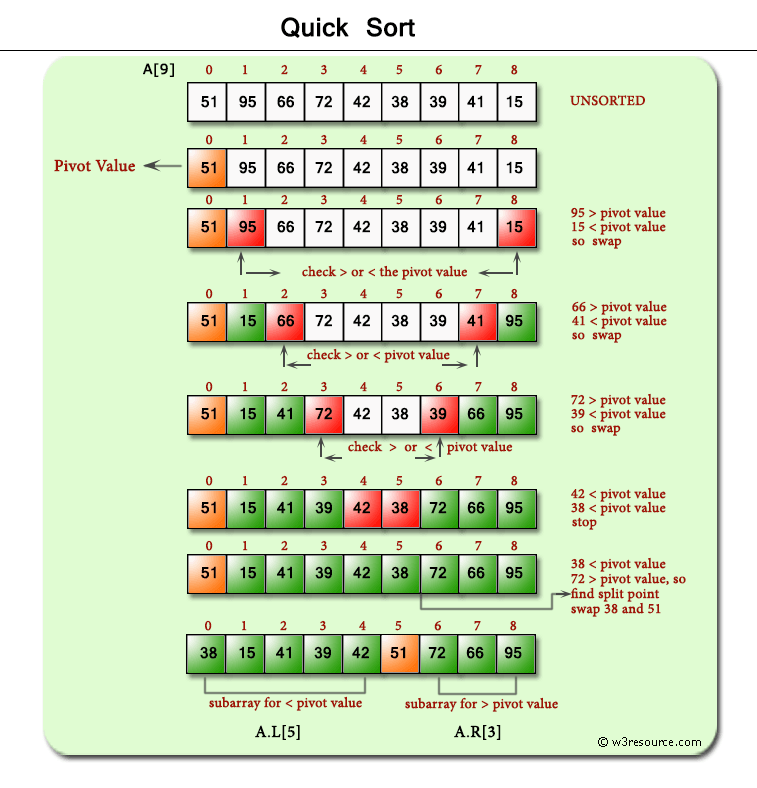
\includegraphics[width=15cm]{img/quick_sort.png}

\begin{code}
Partition(tab, left, right)
	pivot = tab[left]
    i = left - 1
    j = right
    Tant que ( vrai ) :
    	// On trouve une valeur qui doit passer à droite
    	Faire
        	i = i + 1
        	tant que (tab[i] < pivot)
        // On  trouve une valeur qui doit passer à gauche
        Faire
        	j = j - 1
        	tant que (tab[j] > pivot)
       	// Si la partie de droite passe à gauche alors c'est fini
       	Si (j <= i)
        	Si (i == left)
            	retourner i + 1
            Sinon
            	retourner i
       tmp = tab[i] // on échange tab[i] et tab[j]
       tab[i] = tab[j]
       tab[j] = tmp
\end{code}

\begin{code}
QuickSort(tab, right, left)
	Si (right - left > 1)
    	p = Partition(tab, left, right)
        QuickSort(tab, left, p)
        QuickSort(tab, p, right)
\end{code}

A vous de traduire maintenant :

\begin{code}
static int partition(int[] array, int left, int right)
{
	// TODO
    return 0;
}
\end{code}

\begin{code}
static void quick_sort(int[] array, int left, int right)
{
	// TODO
}
\end{code}

\underline{Tips} : Vous pouvez tester \texttt{Quick Sort} à l'aide de \texttt{print\_array()}.


